\documentclass[pdflatex,sn-nature]{sn-jnl}

%%%% Standard Packages
\usepackage{graphicx}%
\usepackage{multirow}%
\usepackage{amsmath,amssymb,amsfonts}%
\usepackage{booktabs}%
\usepackage{array}%
\usepackage{xcolor}%
\usepackage{textcomp}%

\raggedbottom
\begin{document}
\title[BorderRPV]{Economic returns and policy frictions, not wealth, shape rooftop solar divergence in neighboring border cities}

\author*[1]{\fnm{Yue} \sur{Zhuo}}
\author*[1,2,3]{\fnm{Fengqi} \sur{You}}\email{fengqi.you@cornell.edu}

\affil*[1]{\orgdiv{College of Engineering}, \orgname{Cornell University}, \orgaddress{\city{Ithaca, New York 14853}, \country{USA}}}
\affil[2]{\orgdiv{Cornell University AI for Science Institute}, \orgname{Cornell University}, \orgaddress{\city{Ithaca, New York 14853}, \country{USA}}}
\affil[3]{\orgdiv{Cornell AI for Sustainability Initiative (CAISI)}, \orgname{Cornell University}, \orgaddress{\city{Ithaca, New York 14853}, \country{USA}}}


\abstract{
Rooftop photovoltaics (PV) are often treated as a function of solar potential or urban wealth, yet neighboring cities can convert similar rooftop opportunity into markedly different deployment outcomes. Here we compare building-level rooftop PV adoption, project economics and policy frictions across six border-city pairs. Across Vienna--Bratislava, Singapore--Johor Bahru, San Diego--Tijuana, El Paso--Juarez, Hong Kong--Shenzhen and Monaco--Nice, rooftop PV divergence resolves into three recurring patterns: system-wide leadership, income reversal and residential--non-residential segmental divergence. System-wide leaders combine higher PV utilization with stronger returns and equal or lower policy friction: Vienna, Singapore and San Diego exceed their paired neighbors in all-building PV utilization by 1.96, 5.99 and 2.03 percentage points, alongside IRR advantages of 5.35, 22.54 and 9.20 percentage points. By contrast, El Paso has the higher income ranking but lower all-building PV utilization than Juarez, 0.55\% versus 0.76\%, together with a lower IRR and higher total policy friction. Segmental cases further show that residential and non-residential rooftops do not follow a common adoption logic: Hong Kong and Monaco lead their neighbors in residential PV utilization, whereas Shenzhen and Nice lead in non-residential utilization. This segmental pattern extends to large rooftops: among roofs larger than 1,000 m$^2$, Juarez, Shenzhen and Nice outperform their higher-income or residential-leading neighbors. These results show that urban solar readiness is not wealth-determined, but shaped by policy-adjustable return conditions, revenue rules and administrative frictions.}
\maketitle

% =========================
% Main text
% =========================

\section{Introduction}

Cities are increasingly expected to deliver the energy transition from within the existing built environment. Among urban low-carbon technologies, rooftop photovoltaics (PV) are distinctive because they convert already-developed roof space into distributed electricity generation, avoiding additional land competition while placing clean-energy infrastructure close to demand. Global and regional assessments have shown that rooftop PV could make a substantial contribution to electricity supply and climate mitigation, and recent building-level datasets have strengthened the ability to evaluate this potential at scales relevant to urban planning and policy. \cite{RN1,RN2,RN3,RN7,RN31} Yet the urban value of rooftop PV is not determined by technical potential alone. It depends on whether physically available roof area is translated into installed systems through markets, regulations, ownership structures and local implementation capacity. \cite{RN4,RN5,RN6}

A growing literature has therefore shifted from estimating rooftop solar potential to explaining uneven deployment. Remote-sensing and machine-learning approaches have made it possible to map existing PV systems at high spatial resolution, revealing where rooftop solar is adopted and where it remains absent. \cite{RN8,RN9,RN10,RN11,RN28,RN29} Parallel work has shown that rooftop PV adoption is socially and institutionally uneven: income, home ownership, race and ethnicity, peer effects, financing models and policy interventions all shape who benefits from distributed solar. \cite{RN12,RN13,RN15,RN16,RN17,RN21,RN22,RN23} More recent evidence also suggests that residential and non-residential rooftops should not be treated as a single adoption category, because their deployment patterns, decision makers and policy sensitivities can differ substantially. \cite{RN18,RN19,RN20}

Despite these advances, an important urban-comparative question remains unresolved: why do neighboring cities with similar geography and regional exposure sometimes follow sharply different rooftop PV trajectories? Much of the existing evidence is organized within national or subnational policy systems, where climate, institutions and market conditions are often examined together. This makes it difficult to separate broad wealth gradients from more proximate deployment conditions such as electricity value, export compensation, permitting complexity, interconnection procedures and other administrative frictions. Border-city regions provide a useful setting for this problem. Cities on opposite sides of a border may be geographically close and physically comparable, yet they are embedded in different regulatory, market and governance systems. Such settings allow rooftop PV divergence to be examined not only as a difference in solar resource or urban wealth, but as an outcome of economic returns and policy-adjustable frictions.

Here we use six neighboring border-city pairs to examine how rooftop PV adoption diverges across adjacent urban systems. We combine building-level rooftop PV mapping with city-level indicators of economic return and policy friction, then compare these dimensions across Vienna--Bratislava, Singapore--Johor Bahru, San Diego--Tijuana, El Paso--Ciudad Juarez, Hong Kong--Shenzhen and Monaco--Nice. Fig.~\ref{fig:framework} summarizes the workflow: high-resolution orthophotos are used to map rooftop PV at the building scale; mapped systems are aligned with building footprints and rooftop categories; and deployment outcomes are interpreted alongside socioeconomic, economic and administrative indicators. \cite{RN8,RN9,RN25,RN26,RN28,RN29,RN30} This design asks whether cross-border differences in rooftop PV utilization align more closely with income, project-level returns or policy frictions, and whether these relationships vary between residential and non-residential rooftops.
This paper makes three contributions:
\begin{enumerate}
    \item It provides a building-level, cross-border assessment of rooftop PV deployment across neighboring urban systems. By combining high-resolution rooftop PV mapping with building-footprint alignment, the study enables direct comparison of realized rooftop solar adoption across municipal and national boundaries, rather than relying only on city-scale technical potential or aggregate capacity statistics.

    \item It develops a return-versus-friction framework for explaining rooftop PV divergence. Instead of treating urban wealth as the primary proxy for solar readiness, the analysis links adoption gaps to project-level economic returns, revenue-side conditions and administrative frictions that shape whether rooftop PV is investable, legible and deployable.

    \item It shows that rooftop PV divergence is segment-specific rather than uniform across the built environment. The results distinguish system-wide leadership, income reversal and residential--non-residential divergence, showing that residential and non-residential rooftops can respond to different policy logics even within the same neighboring-city pair.
\end{enumerate}

Based on these findings, we summarize the recommendations to stakeholders:
\begin{enumerate}
    \item Urban governments should move beyond wealth-based or one-size-fits-all solar targets. Rooftop PV policy should be designed around the specific economic and administrative barriers that limit deployment in each city, including electricity value, export compensation, permitting procedures and interconnection requirements.

    \item Energy regulators and utilities should treat revenue design as a core urban solar policy instrument. Export rates, compensation rules and grid-connection procedures can materially affect project returns, especially where technical rooftop potential exists but deployment remains low.

    \item City planners should differentiate residential and non-residential rooftop strategies. Household PV adoption may require targeted financing, ownership and equity-oriented support, whereas non-residential and large-roof deployment may depend more strongly on project aggregation, streamlined approvals, commercial tariffs and grid-access clarity.

    \item Lower-adoption border cities should prioritize policy-adjustable frictions rather than assuming that adoption will rise automatically with income growth. The cross-border comparisons suggest that procedural simplification, transparent approval pathways and improved project economics can be more actionable levers than broad socioeconomic development alone.

    \item Researchers and data providers should build comparable, building-level rooftop PV datasets across jurisdictions. Standardized cross-border mapping can help identify where adoption gaps reflect physical constraints, economic returns, policy frictions or segment-specific opportunity structures.
\end{enumerate}

\begin{figure}[t]
\centering
\includegraphics[width=\textwidth]{../figures/main/fig_1.pdf}
\caption{\textbf{Cross-border rooftop PV mapping links building-scale deployment to pairwise economic and policy comparisons.} \textbf{a, The mapping workflow combines orthophoto collection, SegFormer-based visual modelling, PV segmentation, building-footprint integration and building-level rooftop PV alignment.} The panel reports 327k images, 5,822 km$^2$ land area, 3.8M buildings, 704 km$^2$ rooftop area, and test-set Dice and IoU ranges of 0.823--0.956 and 0.707--0.896, respectively. \textbf{b, Rooftop PV heatmaps show the spatial intensity of mapped systems across the six border-city pairs.} Heatmaps are shown as Gaussian-smoothed spatial intensity surfaces (smoothing sigma = 8 pixels), with a world locator map indicating study locations. \textbf{c, City-level socioeconomic, economic and policy-friction variables provide the comparative inputs for downstream analysis.} \textbf{d, The neighboring-city divergence framework organizes mapped deployment into recurring patterns, factor comparisons and policy interpretation.} Together, the workflow shows how building-scale PV mapping feeds the pairwise economic and policy comparisons used throughout the paper.}
\label{fig:framework}
\end{figure}

\section{Results}

\subsection{Border-city rooftop PV adoption diverges through three recurring patterns}

Neighboring border cities do not converge toward a common level of rooftop PV adoption, despite their geographic proximity. Instead, the six pairs resolve into three recurring patterns: system-wide leadership by one city, income reversal, and segmental divergence between residential and non-residential rooftops (Fig.~\ref{fig:patterns}a,b). This pattern-based structure is visible when all-building PV utilization is read alongside residential and non-residential utilization within each pair. It provides the organizing logic for the Results section, allowing the analysis to compare recurring cross-border outcomes rather than follow the figures sequentially. The pattern indicates that the border-city solar gap is not a single monotonic gradient, but a repeated set of contrasts that must be interpreted at the pair and segment levels.

System-wide leadership occurs where the same city leads across all rooftop segments. Vienna exceeds Bratislava for all buildings (2.77\% vs.\ 0.81\%), residential buildings (1.73\% vs.\ 0.65\%) and non-residential buildings (3.89\% vs.\ 0.91\%); Singapore similarly leads Johor Bahru across the same three measures (7.28\% vs.\ 1.29\%, 4.05\% vs.\ 0.26\% and 8.93\% vs.\ 2.10\%); and San Diego leads Tijuana for all buildings (2.63\% vs.\ 0.60\%), residential buildings (2.69\% vs.\ 0.15\%) and non-residential buildings (2.60\% vs.\ 1.30\%) (Fig.~\ref{fig:patterns}a). These cases show that a city-wide PV advantage can extend across both residential and non-residential rooftops, providing a baseline pattern against which more divergent pair structures can be compared.

Income advantage is not sufficient to predict rooftop PV leadership. El Paso has the higher income ranking within its pair, yet Juarez has higher overall PV utilization (0.76\% vs.\ 0.55\%) and residential PV utilization (1.34\% vs.\ 0.71\%), while the non-residential contrast is smaller (0.70\% vs.\ 0.53\%) (Fig.~\ref{fig:patterns}a,b). Because the rank comparison places income and PV utilization on opposite sides of the border, this pair directly challenges a simple wealth-gradient interpretation. The income-reversal pattern cautions against treating city wealth as a direct proxy for rooftop PV uptake. It also motivates the later comparison of project returns and policy frictions as more proximate conditions associated with deployment.

Segmental divergence reveals a third form of cross-border asymmetry, in which the leading city depends on building type. Shenzhen has higher overall and non-residential PV utilization than Hong Kong (2.81\% vs.\ 1.87\% overall; 3.69\% vs.\ 2.48\% non-residential), whereas Hong Kong remains higher in the residential segment (1.12\% vs.\ 0.71\%) (Fig.~\ref{fig:patterns}a). Nice shows a similar split relative to Monaco, leading slightly overall (0.83\% vs.\ 0.79\%) and in non-residential buildings (1.12\% vs.\ 0.65\%), while Monaco leads in residential buildings (0.96\% vs.\ 0.19\%). The repeated appearance of system-wide leadership, income reversal and segmental divergence shows that cross-border rooftop PV gaps are structured rather than idiosyncratic, setting up the paper's broader argument that economic returns, policy frictions and rooftop segments jointly shape urban PV divergence.

\begin{figure}[t]
\centering
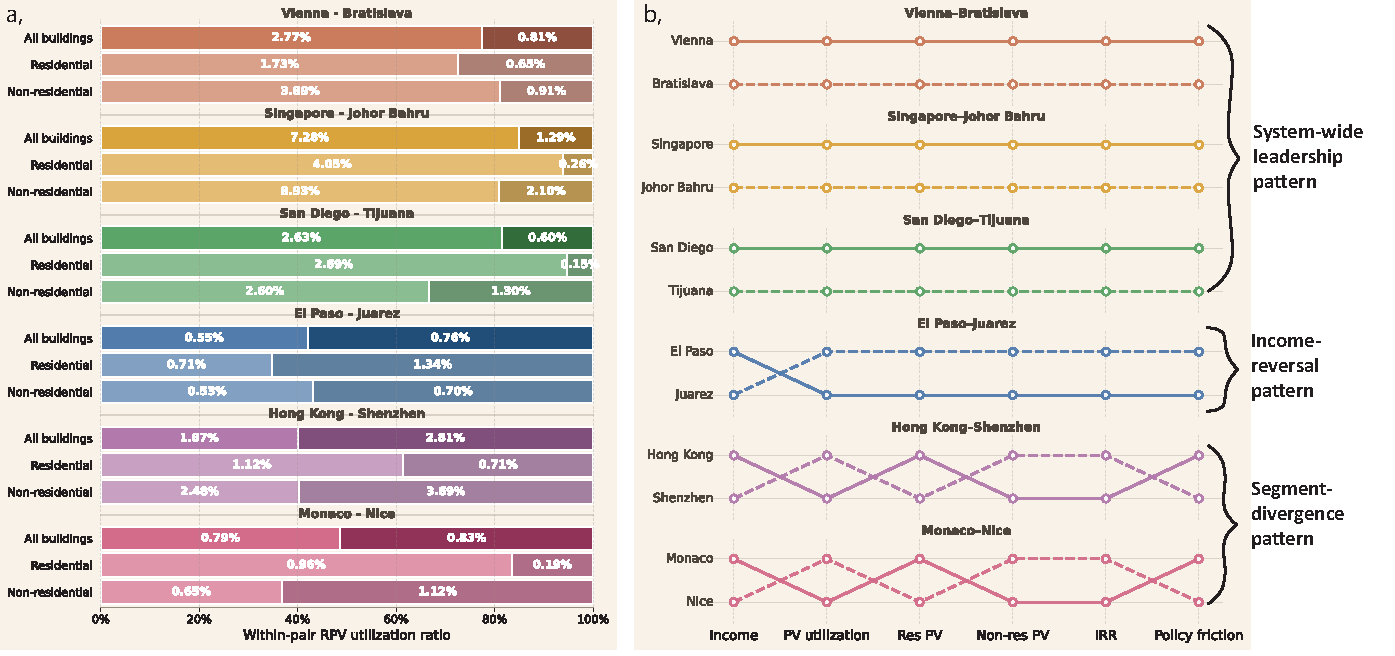
\includegraphics[width=\textwidth]{../figures/main/fig_2.pdf}
\caption{\textbf{Neighboring border cities diverge through recurring rooftop PV adoption patterns rather than a single wealth gradient.} \textbf{a, Within-pair PV utilization separates system-wide leadership, income reversal and segmental divergence.} Horizontal bars compare all-building, residential and non-residential rooftop PV utilization for each border-city pair, with printed percentages reporting the city-level utilization values. \textbf{b, Rank comparisons show that PV leadership does not consistently follow income leadership.} Within-pair ranks are compared across income, PV utilization, residential PV, non-residential PV, internal rate of return (IRR) and policy friction; higher ranks indicate higher income, PV utilization and IRR, whereas lower friction is the more favorable condition. The grouped line patterns classify the six pairs as system-wide leadership (Vienna--Bratislava, Singapore--Johor Bahru and San Diego--Tijuana), income reversal (El Paso--Juarez) and segmental divergence (Hong Kong--Shenzhen and Monaco--Nice).}
\label{fig:patterns}
\end{figure}

\subsection{Overall PV gaps align more closely with differences in economic returns and policy frictions than with wealth}

All-building PV gaps are more closely associated with project economics and policy friction than with income alone. The three system-wide leadership pairs all place the first-listed city in the direction of stronger returns and equal or lower total policy friction: Vienna--Bratislava has an IRR gap of 5.35 percentage points and a total-friction gap of $-3$, Singapore--Johor Bahru has an IRR gap of 22.54 percentage points and a total-friction gap of $-11$, and San Diego--Tijuana has an IRR gap of 9.20 percentage points and a total-friction gap of $-1$ (Fig.~\ref{fig:gap_drivers}a). El Paso--Juarez reverses this structure: El Paso has the income advantage, but its IRR gap is $-6.70$ percentage points, its total-friction gap is $+3$, and the all-building PV gap favors Juarez. These contrasts indicate that wealth ranking alone does not consistently identify the city with stronger rooftop PV adoption.

The pair-level factor comparisons reinforce this interpretation. Across the six pairs, the fitted relationship between income gap and PV utilization gap is shallow, whereas the IRR comparison shows a stronger positive pattern and the total-friction comparison shows a negative pattern, consistent with larger PV gaps where returns are stronger and friction is lower (Fig.~\ref{fig:gap_drivers}b). The decomposition by friction component further shows that the strongest system-wide leaders combine return advantages with lower administrative and revenue frictions: Singapore has gaps of 22.54 percentage points in IRR, $-3$ in administrative friction and $-8$ in revenue friction relative to Johor Bahru, while Vienna has corresponding gaps of 5.35 percentage points, $-1$ and $-2$ relative to Bratislava (Fig.~\ref{fig:gap_drivers}c). San Diego's leadership is also associated with a positive IRR gap and lower administrative friction, although its revenue-friction gap runs in the opposite direction. These mixed component patterns suggest that return and friction conditions operate jointly rather than through a single universal pathway.

City-level economic indicators clarify why similar levels of wealth can translate into different PV outcomes. The most favorable combinations of NPV and IRR occur in San Diego and Singapore, whereas El Paso is the weakest economic case (Fig.~\ref{fig:econ_contrasts}a). Over the 25-year discounted cash-flow horizon, cumulative discounted cash flow reaches \$19,047.70 in San Diego and \$16,602.89 in Singapore, compared with only \$402.50 in El Paso, and the plotted trajectories now include uncertainty intervals around each city path (Fig.~\ref{fig:econ_contrasts}b). These returns reflect the spread between blended solar value and LCOE, together with electricity and export-rate structures: San Diego combines \$0.282~kWh$^{-1}$ in blended solar value with a \$0.1103~kWh$^{-1}$ LCOE, Singapore combines \$0.234~kWh$^{-1}$ with \$0.0641~kWh$^{-1}$, and El Paso is nearly at parity (\$0.097 versus \$0.0936~kWh$^{-1}$), with uncertainty bars shown on the value and rate comparisons (Fig.~\ref{fig:econ_contrasts}c). The economic comparison therefore points to realized project returns, rather than income alone, as a proximate condition associated with all-building PV leadership.

Policy-friction contrasts complement the return-side evidence by showing where deployment and monetization conditions are more or less enabling. The lower-friction side is also the all-building PV leader in Vienna--Bratislava (total friction 7 versus 10), Singapore--Johor Bahru (9 versus 20) and San Diego--Tijuana (6 versus 7), while the income-reversal pair again points in the opposite direction because El Paso has higher total friction than Juarez (10 versus 7) (Fig.~\ref{fig:friction_matrix}). Hong Kong--Shenzhen and Monaco--Nice are more complex: Hong Kong and Monaco have lower revenue friction than their counterparts, yet Shenzhen and Nice lead overall and in non-residential utilization. Taken together, the return and friction evidence supports a broader argument that cross-border rooftop PV divergence is associated with policy-adjustable economic and institutional conditions, not simply with the wealth ranking of neighboring cities.

\begin{figure}[t]
\centering
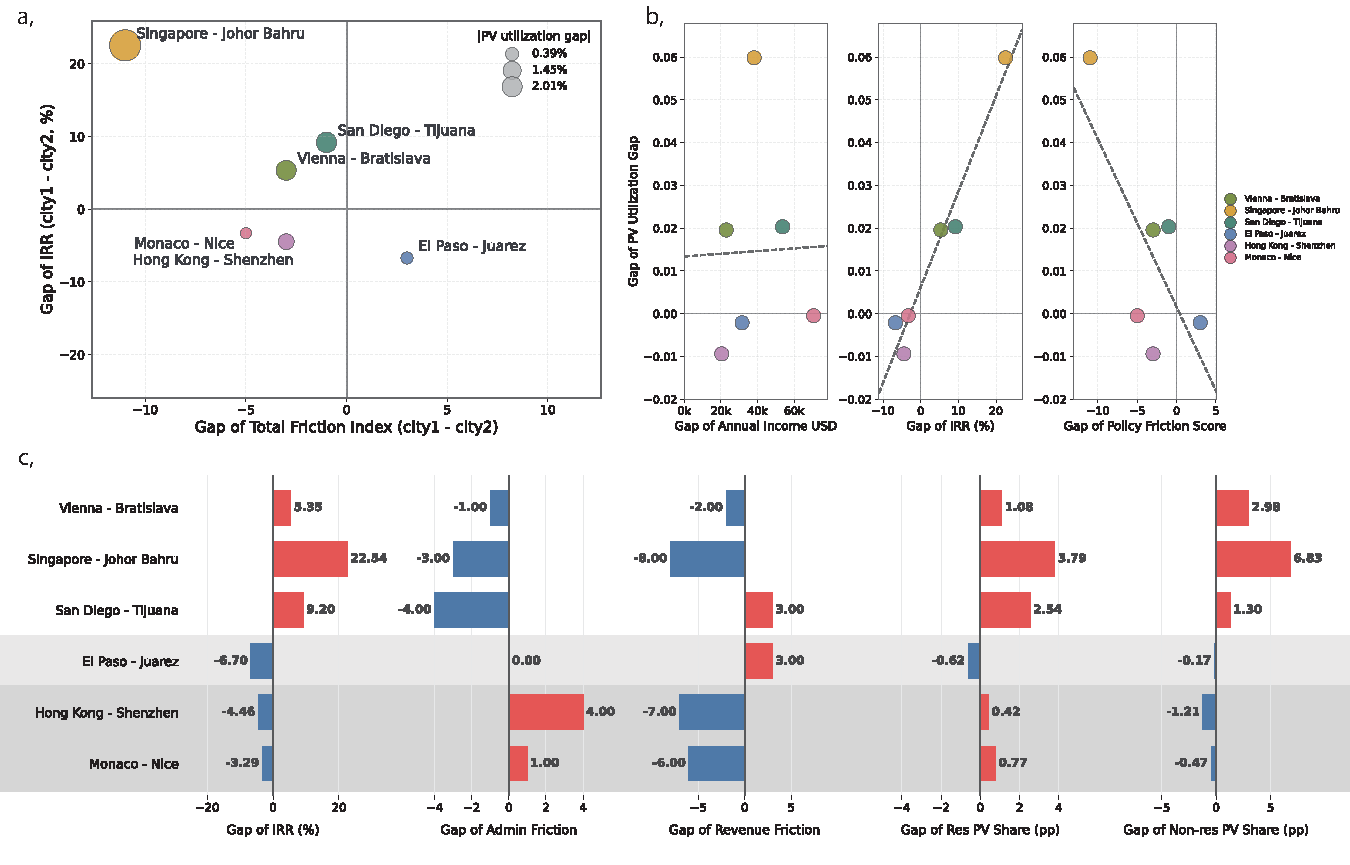
\includegraphics[width=\textwidth]{../figures/main/fig_3.pdf}
\caption{\textbf{Pair-level PV utilization gaps align more consistently with economic-return and policy-friction differences than with income alone.} \textbf{a, Return and friction gaps jointly locate the direction and magnitude of all-building PV divergence.} The scatter compares signed total policy-friction gaps (city1 -- city2) with signed IRR gaps, with bubble size encoding the absolute all-building PV utilization gap. \textbf{b, Cross-factor comparisons show a weaker income relationship than the return and friction relationships.} The same signed PV utilization gap is plotted against annual income gap, IRR gap and total policy-friction score gap, with dashed fitted trend lines shown for visual comparison. \textbf{c, Residential and non-residential PV components do not always move together.} Signed pair-level gaps are shown for IRR, administrative friction, revenue friction, residential PV share and non-residential PV share; residential and non-residential PV gaps are reported in percentage points (pp).}
\label{fig:gap_drivers}
\end{figure}

\begin{figure}[t]
\centering
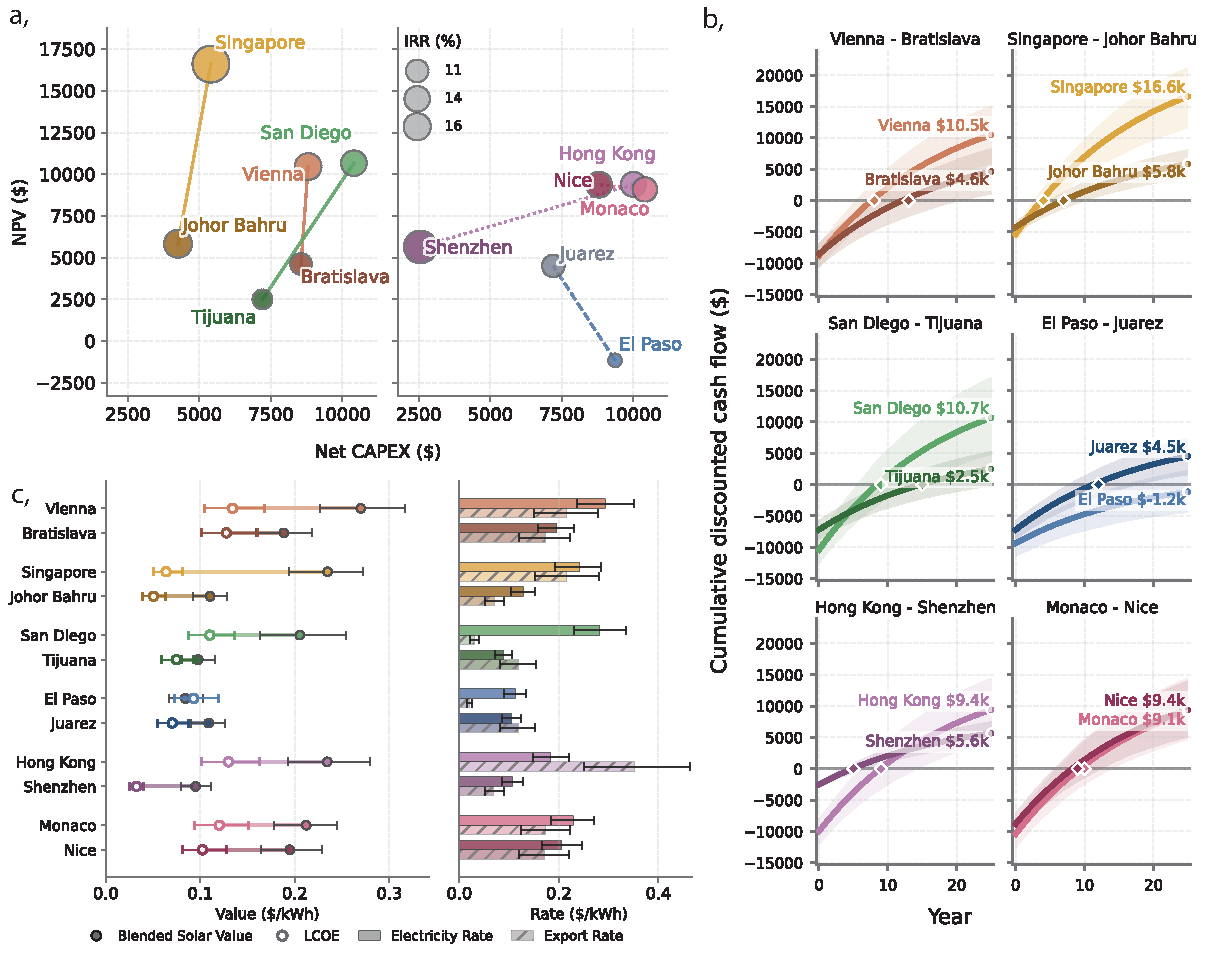
\includegraphics[width=\textwidth]{../figures/main/fig_4.pdf}
\caption{\textbf{Cross-border rooftop PV economics differ through capital cost, long-run returns and local rate structures.} \textbf{a, Net capital expenditure and profitability vary sharply across neighboring cities.} The scatter compares net capital expenditure (CAPEX) and net present value (NPV) for the 12 cities, with marker area scaled by IRR and lines linking cities within each border pair; the corresponding error-bar version is provided in Supplementary Fig.~\ref{fig:s2_economic_uncertainty_capex_npv}. \textbf{b, Discounted cash-flow trajectories show how profitability accumulates over a 25-year project lifetime.} Curves are generated under the same model structure and show cumulative discounted cash flow by city with 95\% confidence intervals. \textbf{c, Value-to-cost spreads and rate structures explain the direction of return differences.} The left panel shows city-level dumbbells between blended solar value and levelized cost of electricity (LCOE), while the right panel shows electricity and export rates under the same city ordering, with 95\% confidence intervals on both value and rate components.}
\label{fig:econ_contrasts}
\end{figure}

\begin{figure}[t]
\centering
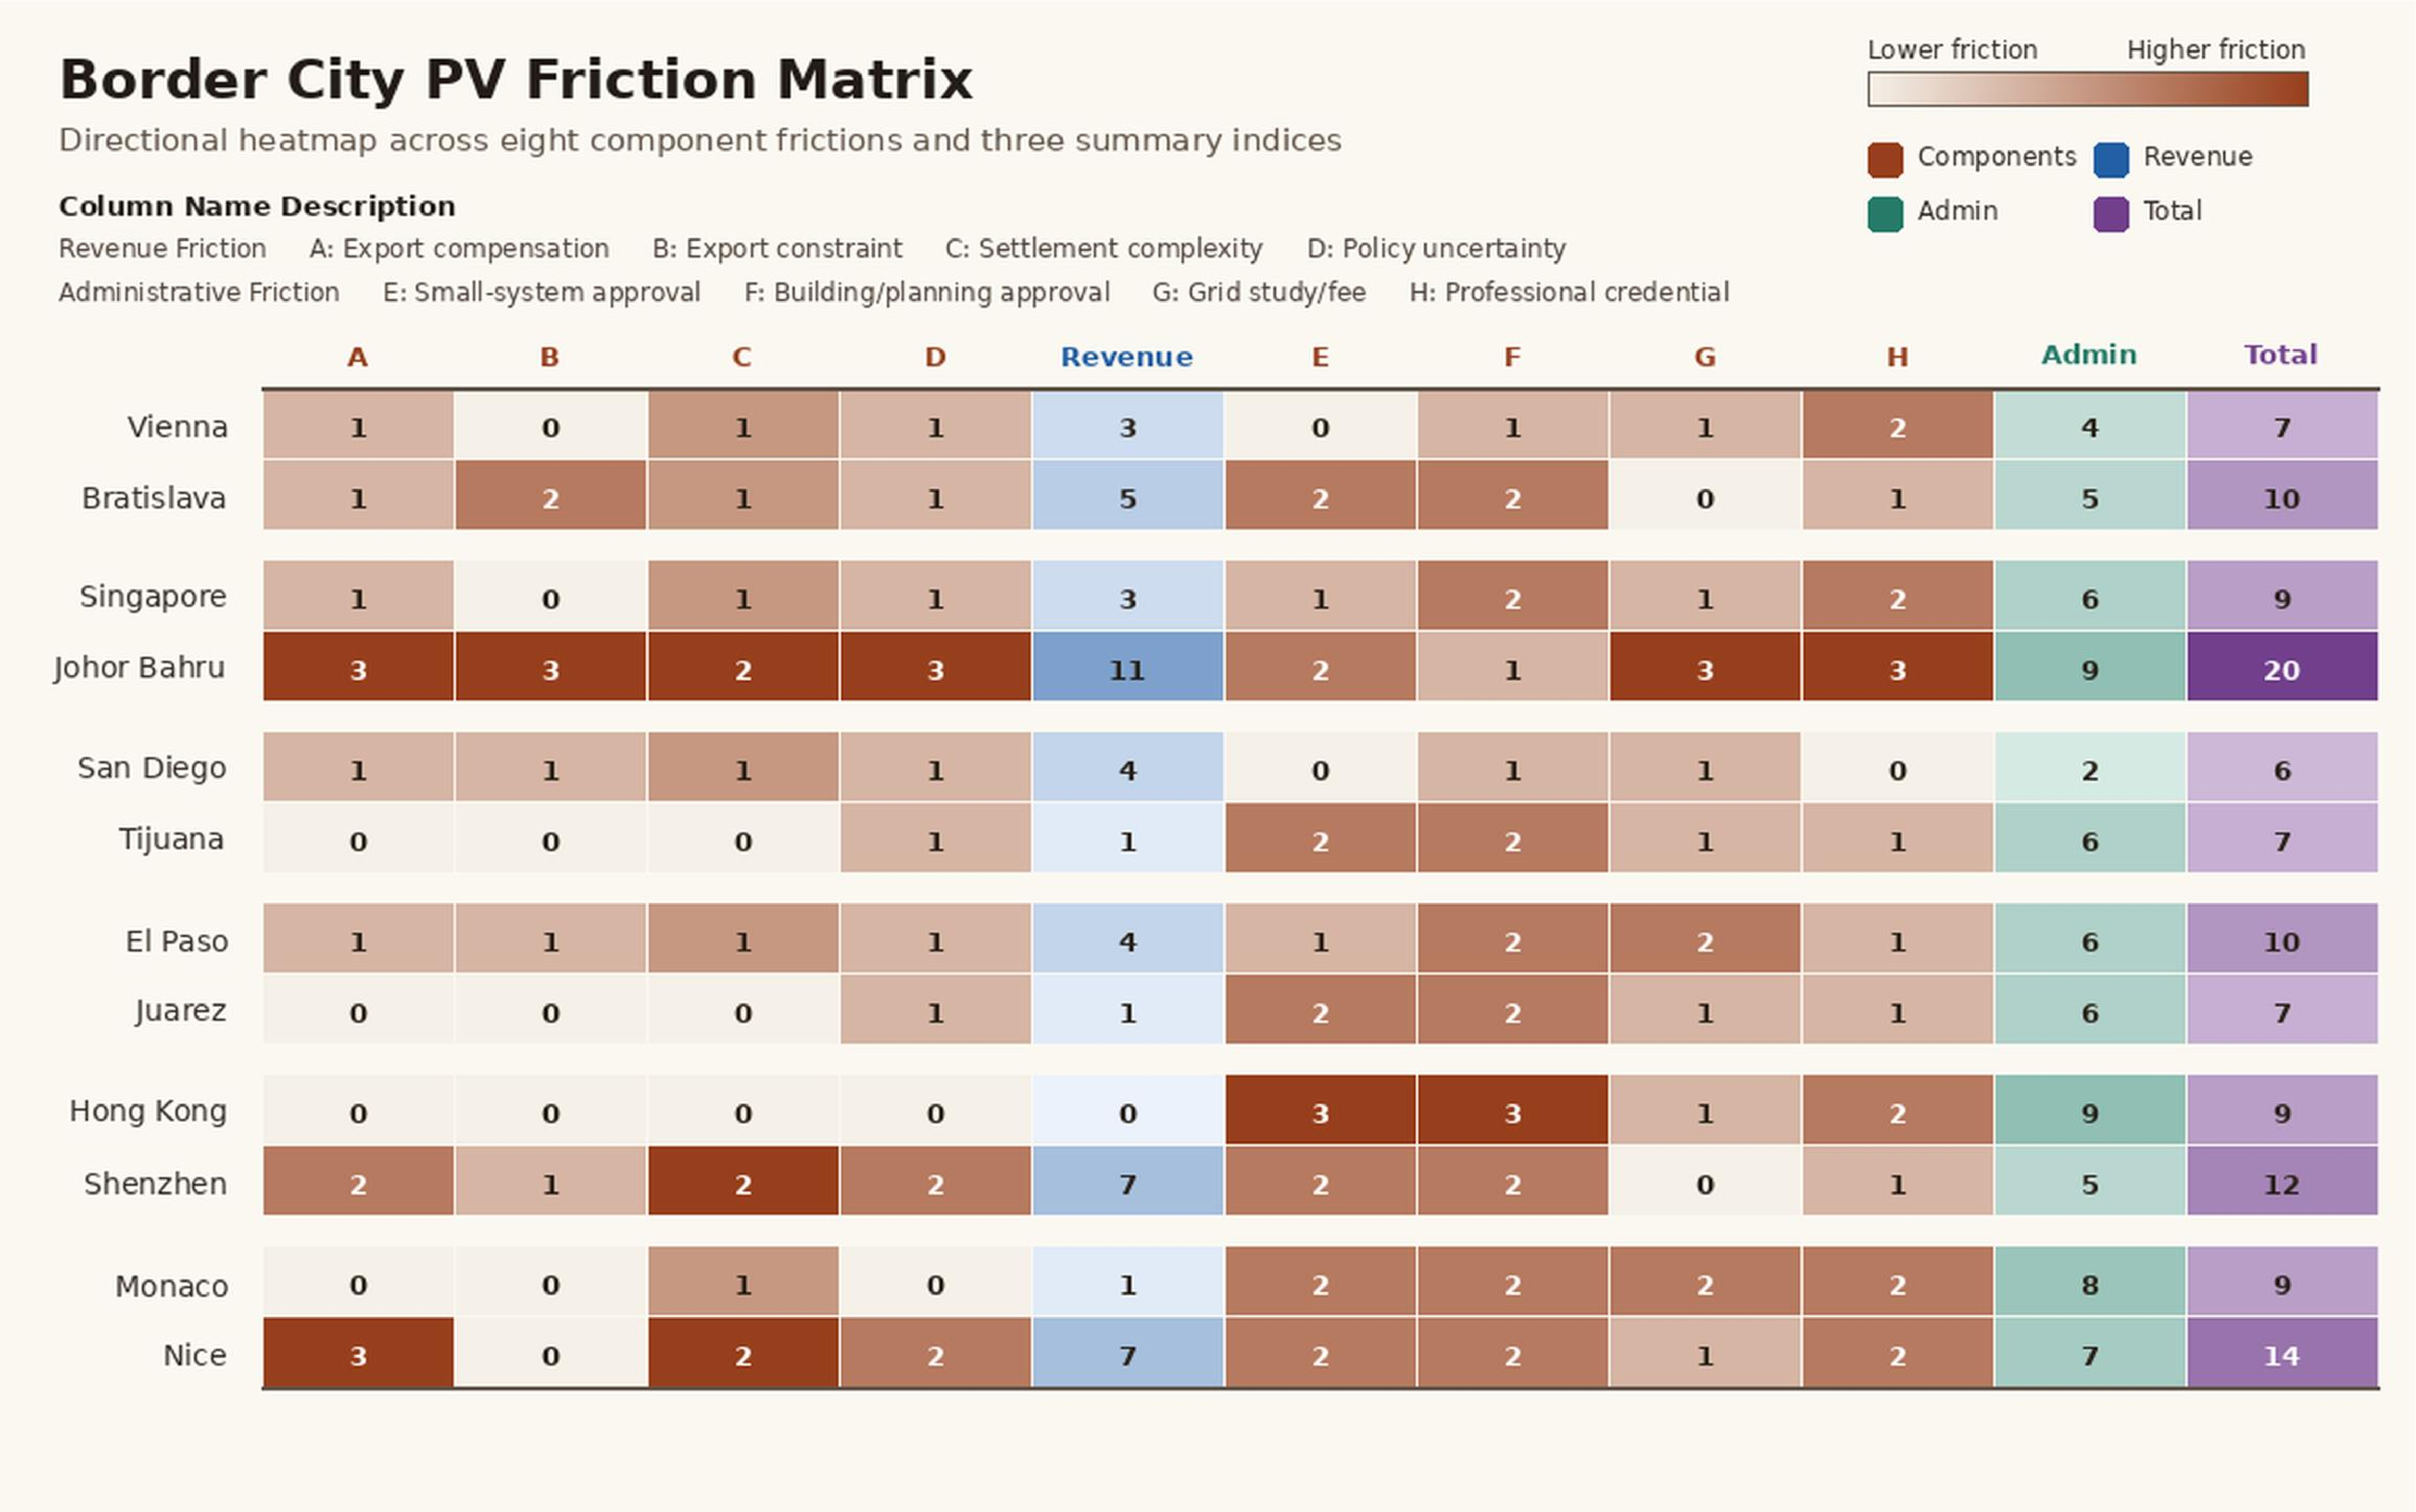
\includegraphics[width=\textwidth]{../figures/main/fig_5.pdf}
\caption{\textbf{Revenue-side and administrative policy frictions vary substantially across neighboring border cities.} The heatmap reports eight component frictions and three summary indices for each city side of the six border-city pairs. Components are scored from 0 (lowest friction) to 3 (highest friction) and include export compensation (A), export constraint (B), settlement complexity (C), policy uncertainty (D), small-system approval (E), building or planning approval (F), grid study or fee (G), and professional credential (H). Summary columns aggregate revenue friction, administrative friction and total friction. The matrix distinguishes monetization barriers from procedural barriers, supporting the manuscript's separation of revenue-side and administrative constraints on rooftop PV deployment.}
\label{fig:friction_matrix}
\end{figure}

\subsection{Segmental divergence reveals distinct policy logics across building types}

Aggregate PV gaps conceal segment-specific patterns that are central to the cross-border divergence observed here. In the three system-wide leadership pairs, residential and non-residential gaps have the same sign but different magnitudes: Vienna--Bratislava has gaps of 1.08 and 2.98 percentage points, Singapore--Johor Bahru has gaps of 3.79 and 6.83 percentage points, and San Diego--Tijuana has gaps of 2.54 and 1.30 percentage points, respectively (Fig.~\ref{fig:gap_drivers}c). El Paso--Juarez is negative in both segments ($-0.62$ and $-0.17$ percentage points), consistent with the income-reversal pattern. The strongest evidence for distinct segmental logics comes from Hong Kong--Shenzhen and Monaco--Nice, where residential gaps favor Hong Kong and Monaco (+0.42 and +0.77 percentage points), but non-residential gaps favor Shenzhen and Nice ($-1.21$ and $-0.47$ percentage points).

Large-roof and building-use patterns show where the segmental divergence is concentrated. In the largest roof-size bin (1000+~m$^{2}$), the lower-income city leads in El Paso--Juarez (Juarez 1.92\% vs.\ El Paso 0.31\%), Hong Kong--Shenzhen (Shenzhen 3.46\% vs.\ Hong Kong 2.17\%) and Monaco--Nice (Nice 2.01\% vs.\ Monaco 1.05\%) (Fig.~\ref{fig:segment_heterogeneity}a). Even where San Diego remains the system-wide leader, the large-roof contrast with Tijuana narrows to 2.74\% versus 2.48\%. Building-use classes provide the same signal in a different form: Hong Kong leads Shenzhen in single-residential adoption (4.01\% vs.\ 1.33\%), but Shenzhen is higher in commercial (8.99\% vs.\ 3.57\%) and industrial buildings (9.29\% vs.\ 4.77\%) (Fig.~\ref{fig:segment_heterogeneity}b). These patterns indicate that rooftop opportunity structure and building type can redirect PV leadership even within the same neighboring-city pair.

The policy-friction matrix is consistent with residential and non-residential deployment responding to different policy conditions. In Hong Kong--Shenzhen and Monaco--Nice, the residential-leading city has lower revenue friction (Hong Kong 0 versus Shenzhen 7; Monaco 1 versus Nice 7), even though it does not have lower administrative friction (Hong Kong 9 versus Shenzhen 5; Monaco 8 versus Nice 7) (Fig.~\ref{fig:friction_matrix}). El Paso--Juarez shows a similar revenue-side contrast, with Juarez combining lower revenue friction (1 versus 4) with higher residential PV utilization. These comparisons do not establish a single causal mechanism, but they are consistent with residential PV being more closely associated with revenue-side rules, while large-roof and non-residential PV are also shaped by administrative conditions and rooftop opportunity structures. This segmental evidence strengthens the broader argument that border-city rooftop PV divergence emerges from the interaction of economic returns, policy frictions and building-type heterogeneity.

\begin{figure}[t]
\centering
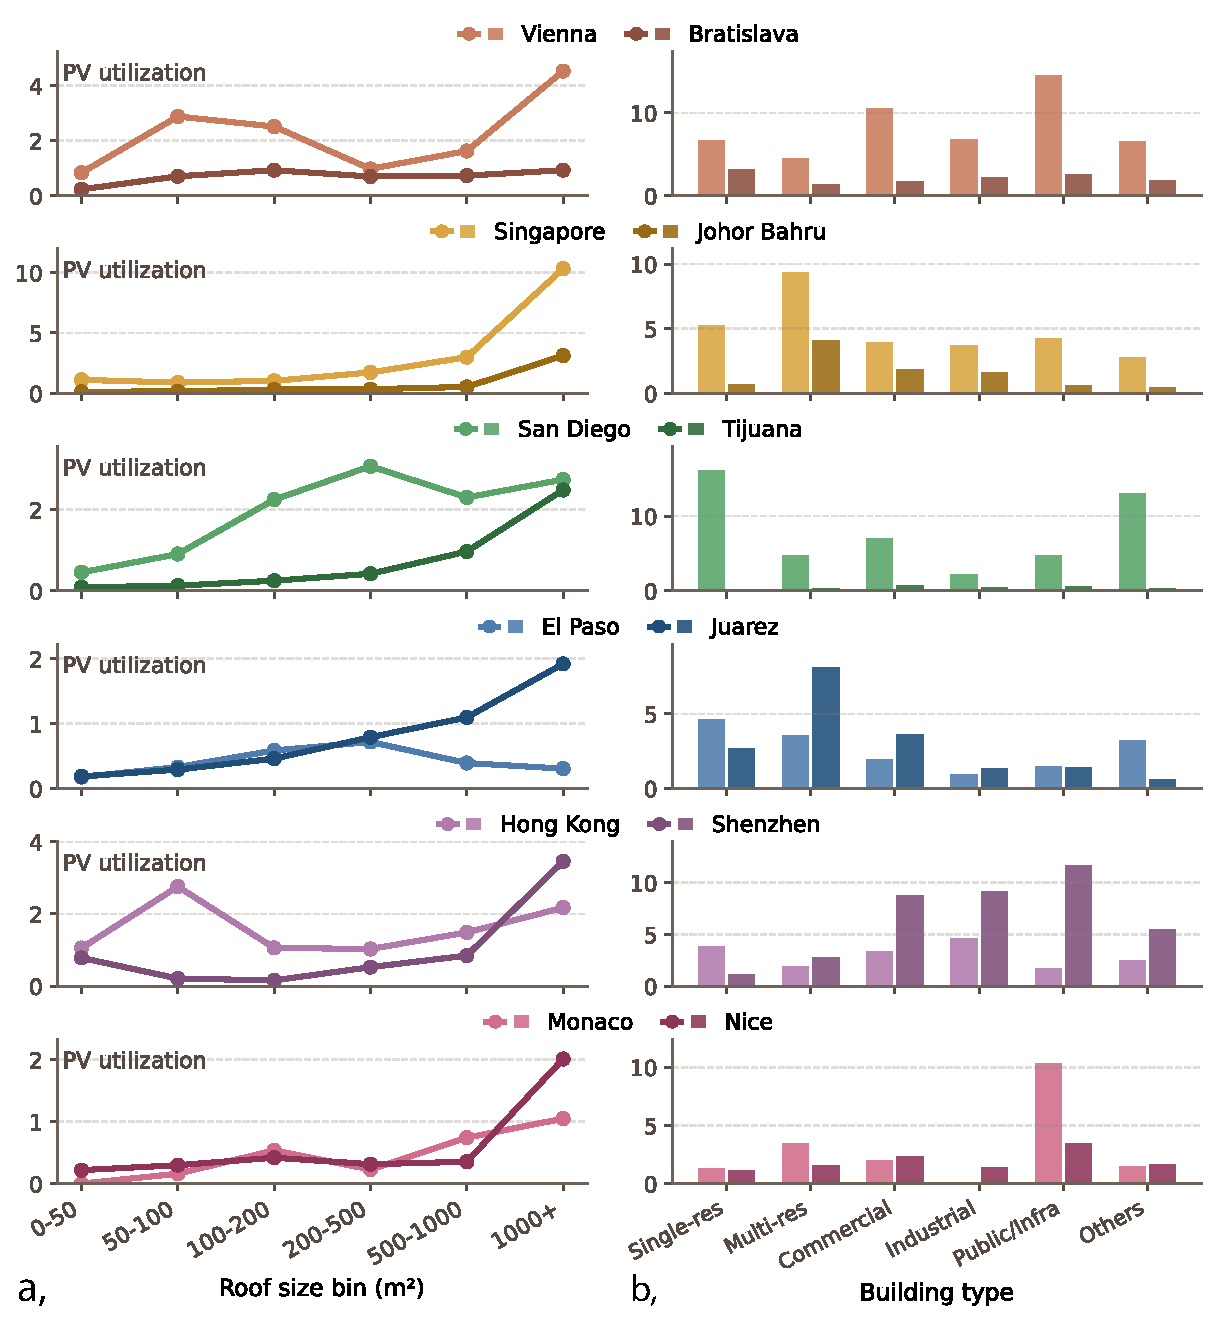
\includegraphics[width=0.8\textwidth]{../figures/main/fig_6.pdf}
\caption{\textbf{Rooftop PV leadership shifts across roof-size bins and building-use classes.} \textbf{a, Large-roof PV utilization can favor lower-income or non-residential-leading cities within a pair.} Lines compare rooftop PV utilization by roof-size bin for each city within the six border-city pairs, showing how relative deployment changes from small roofs to large roofs. \textbf{b, Building-level adoption differs by use class within the same city pair.} Bars report the fraction of buildings in each class with at least one mapped rooftop PV segment. Pairwise leadership is not uniform across rooftop opportunity structures: Juarez, Shenzhen and Nice retain stronger or closer performance in large-roof or non-residential segments relative to their neighboring cities, while the San Diego--Tijuana contrast narrows for larger roofs.}
\label{fig:segment_heterogeneity}
\end{figure}

\section{Discussion}

\emph{Wealth is not destiny: policy-adjustable friction and return conditions shape the solar gap.} The cross-border comparisons suggest that urban solar readiness cannot be inferred from income or macroeconomic status alone. The income-reversal and segmental-divergence cases show that the higher-income city need not lead in overall, residential or non-residential rooftop PV adoption (Fig.~\ref{fig:patterns}). Instead, PV leadership is more closely associated with the conditions that shape project value and deployment feasibility, including return-side factors and policy-friction differences (Fig.~\ref{fig:gap_drivers}; Fig.~\ref{fig:econ_contrasts}; Fig.~\ref{fig:friction_matrix}). This finding matters for policy because many of these conditions are more directly adjustable than urban wealth: tariff design, export compensation, administrative complexity, interconnection procedures and capital-cost support can affect the realized attractiveness of rooftop PV. The implication is not that income is irrelevant, but that wealth is an incomplete proxy for whether urban rooftops can become investable, legible and deployable solar assets.

The IRR catch-up decomposition makes this point more concrete by translating return gaps into the scale of one-factor adjustments that would be needed for a lagging city to match its paired leader. In El Paso--Juarez, for example, the lower-income city has the higher baseline IRR, and matching Juarez's IRR would require El Paso to raise the export rate from \$0.020 to \$0.217~kWh$^{-1}$, or alternatively add a PV subsidy of about \$3,890, equivalent to 33.2\% of gross CAPEX (Supplementary Table~S3). This is not a policy prescription, because actual reform would combine multiple instruments and face local constraints. It does, however, show that the economic distance between paired cities is large enough that modest income differences cannot explain the observed adoption ordering on their own.

\emph{System-wide PV leadership emerges where favorable returns are reinforced by supportive policy environments.} The system-wide leadership cases point to the importance of alignment between economic returns and lower deployment friction. Vienna, Singapore and San Diego lead their neighboring cities across all rooftop segments, and these advantages are associated with stronger return conditions and equal or lower total policy friction (Fig.~\ref{fig:patterns}; Fig.~\ref{fig:gap_drivers}). Their paired economic contrasts are also large in practical terms. Matching the leading-city IRR would require Johor Bahru to close a 22.54 percentage-point IRR gap with Singapore, Tijuana to close a 9.20 percentage-point gap with San Diego, and Bratislava to close a 5.35 percentage-point gap with Vienna (Supplementary Table~S3). These gaps are consistent with Fig.~\ref{fig:econ_contrasts}, where leading cities occupy more favorable positions in value-to-cost and discounted cash-flow space.

The required one-factor adjustments further suggest why system-wide leadership is unlikely to be narrowed by a small change to any single policy margin. Johor Bahru would require an additional export value of \$0.413~kWh$^{-1}$ above its current export rate, or an additional subsidy of about \$2,962, equivalent to 59.2\% of gross CAPEX, to match Singapore's IRR under the table's counterfactual assumptions. Tijuana would require an additional \$0.250~kWh$^{-1}$ export-rate increase or about \$2,933 in additional subsidy to match San Diego, while Bratislava would require an additional \$0.239~kWh$^{-1}$ or about \$2,527 to match Vienna (Supplementary Table~S3). These values indicate that system-wide PV leadership reflects a bundle of favorable return and friction conditions rather than a marginal advantage in one variable. For urban energy transitions, this shifts attention from single-instrument explanations toward the combined architecture of electricity value, export rules, permitting pathways and administrative clarity.

\emph{For lower-adoption border cities, large-roof non-residential PV is a strategic frontier for scaling urban solar.} The segmental results highlight large-roof and non-residential buildings as a distinct policy and infrastructure frontier. Several cities that do not lead across all rooftops perform better, or much closer to their neighbor, in the largest roof-size bins or in commercial and industrial building classes (Fig.~\ref{fig:segment_heterogeneity}). This suggests that lower-adoption cities may have meaningful deployment opportunities outside the household segment, especially where large roofs concentrate technical opportunity and project economics can be evaluated at a more institutional scale. The Hong Kong--Shenzhen and Monaco--Nice pairs are especially instructive because residential leadership and non-residential leadership split across the same border, while El Paso--Juarez and San Diego--Tijuana show that the large-roof gap can narrow or reverse even when the city-wide pattern looks different. The policy relevance is therefore not simply to increase rooftop PV adoption in aggregate, but to recognize that residential and non-residential rooftops face different constraints and may respond to different enabling conditions.

Return-side catch-up requirements also vary substantially across segmental-divergence cases, reinforcing the need for differentiated policy attention. Hong Kong would require an additional export value of \$0.206~kWh$^{-1}$ or an additional subsidy of about \$2,239 to match Shenzhen's IRR, whereas Monaco would require a smaller but still material adjustment of \$0.144~kWh$^{-1}$ or about \$1,649 to match Nice (Supplementary Table~S3). These values sit alongside Fig.~\ref{fig:friction_matrix}, where revenue friction and administrative friction do not always move in the same direction. A residential-oriented policy design that focuses mainly on household compensation rules may therefore miss non-residential bottlenecks related to approvals, grid procedures, roof aggregation or project execution. Conversely, a large-roof strategy that ignores revenue-side settlement and export rules may fail to translate technical opportunity into investable projects.

\emph{Policy implications for broader border-city governance:} The broader implication is that border cities offer a useful lens for understanding how urban decarbonization can diverge under similar geography but different market and institutional settings. The paired-city design shows that neighboring urban systems can follow different rooftop PV trajectories when return conditions, revenue rules, administrative frictions and rooftop opportunity structures differ across the border. The IRR catch-up values extend this insight by showing that the scale of adjustment is highly uneven across pairs: required export-rate increases range from \$0.144 to \$0.413~kWh$^{-1}$, while required additional PV subsidies range from about \$1,649 to \$3,890 across the lagging cities (Supplementary Table~S3). Such variation suggests that a generic rooftop PV policy benchmark is unlikely to travel cleanly across borders. Comparable adoption gaps may require very different combinations of revenue reform, capital-cost support and procedural simplification depending on the local value-to-cost structure.


\emph{Limitations:} Several limitations should guide interpretation of these results. First, the analysis covers six border-city pairs, which provides a structured comparative design but does not establish a globally representative sample of all border cities or urban PV markets. Second, the study is cross-sectional: the observed associations between PV utilization, economic returns and policy friction are consistent with the proposed explanation, but they do not identify policy timing effects or strict causal pathways. Third, the economic model uses standardized system assumptions, tariff inputs and one-factor IRR catch-up counterfactuals, rather than project-specific load profiles, financing terms, installer quotes or owner-level investment decisions; the uncertainty analysis partly tests sensitivity to key inputs, but cannot capture all market heterogeneity. Fourth, the policy-friction indices summarize documented rules and administrative requirements, so they may not fully reflect informal implementation practices, actual approval times, enforcement differences or user experience. Finally, building classification, orthophoto coverage, rooftop PV segmentation and building-footprint alignment can propagate uncertainty into city-level and segment-level utilization metrics. Supplementary Fig.~\ref{fig:s2_economic_uncertainty_capex_npv} retains the detailed uncertainty-propagated CAPEX--NPV comparison, while the main-text Figure~\ref{fig:econ_contrasts} now carries the broader uncertainty presentation. These constraints mean that the results should be read as evidence of recurring cross-border patterns and plausible mechanisms, not as universal estimates of policy effects; broader validation will require additional city pairs, longitudinal policy data and more granular project-level information.

\section{Methods}

\subsection{Rooftop PV segmentation and building-level mapping}

We mapped rooftop PV deployment from orthophoto tiles and linked the resulting PV objects to building footprints before computing city- and segment-level adoption metrics. The workflow comprised supervised PV segmentation, mask vectorization, building-level spatial assignment and building-use harmonization (Fig.~\ref{fig:framework}a). A SegFormer semantic-segmentation model was fine-tuned from a manually labelled border-city annotation pool and then applied to all available orthophoto tiles in the 12 studied cities. The mapped image corpus contained 327,413 orthophoto tiles covering 5,822.3~km$^{2}$ of urban area, while the studied city annotation set contained 623 labelled tiles across the 12 study cities (Supplementary Fig. S1; Supplementary Table S4). This design allowed a common visual model to define the rooftop PV layer before any economic or policy variables entered the analysis.

Rooftop PV identification was treated as a binary semantic-segmentation task. Label masks were converted to binary targets by assigning pixels with grayscale values greater than 127 to the PV class. Supervised fine-tuning used an 80/10/10 train--validation--test split with seed 42, a loss combining binary cross-entropy with logits and Dice loss, a positive-pixel weight of 4.0, and 40 training epochs. The SegFormer encoder was frozen for the first 10 epochs and then updated with a lower learning rate than the decode head ($4\times10^{-5}$ versus $6\times10^{-5}$). During city-scale inference, model logits $z_{i,p}$ for tile $i$ and pixel $p$ were converted to binary PV masks using
\begin{equation}
\hat{M}_{i,p}=\mathbf{1}\left[\sigma(z_{i,p})\geq0.5\right],
\end{equation}
where $\sigma(\cdot)$ is the sigmoid function. Full model, training and inference parameters are reported in Supplementary Table S5.

Predicted PV masks were converted from tile coordinates into georeferenced polygons and merged into city-level PV segment layers. For each mask tile, Mercator tile coordinates were converted to WGS84 tile bounds, an affine transform was constructed from the bounds and mask dimensions, connected PV regions were vectorized, invalid geometries were repaired, and adjacent or overlapping geometries were dissolved. PV segments were then assigned to building footprints by nearest-neighbour matching in EPSG:3857. Segments smaller than 2.5~m$^{2}$ were removed before assignment, and each remaining segment was linked to the nearest building when the distance was no greater than 5~m. The building index and nearest-building distance were retained in the output, so matched PV area could be aggregated by building while unmatched segments remained available for quality checks.

Building footprints were harmonized into six base classes: single-residential, multi-residential, commercial, industrial, public or infrastructure, and others. Single- and multi-residential buildings were grouped as residential, while the remaining mapped classes were grouped as non-residential for the main segment comparisons. For any city or building group $G$, rooftop PV utilization was calculated as
\begin{equation}
U_{G}=\frac{\sum_{b\in G} A^{\mathrm{PV}}_{b}}{\sum_{b\in G} A^{\mathrm{roof}}_{b}},
\end{equation}
where $A^{\mathrm{PV}}_{b}$ is mapped PV area assigned to building $b$ and $A^{\mathrm{roof}}_{b}$ is the building footprint area used as the rooftop-area denominator. Building-type PV adoption was calculated as
\begin{equation}
P_{C}=\frac{1}{N_{C}}\sum_{b\in C}\mathbf{1}\left(A^{\mathrm{PV}}_{b}>0\right),
\end{equation}
where $C$ is a building class and $N_{C}$ is the number of buildings in that class. The same building-level linkage was used for all-building, residential, non-residential, building-type and roof-size comparisons in the Results.

\subsection{PV Economic modeling}

We modelled rooftop PV economics with a standardized discounted cash-flow framework so that neighboring cities could be compared under a common project structure while retaining city-specific cost, tariff and solar-productivity inputs. The model represents a 5~kW rooftop PV system over a 25-year project lifetime with a 5\% discount rate. City-specific inputs included cost per watt, CAPEX reduction, retail electricity rate, export rate, annual PV yield, self-consumption ratio, degradation rate and O\&M rate (Supplementary Table S1). The main-text analysis uses the economic variables shown in Figs.~\ref{fig:patterns}--\ref{fig:econ_contrasts}: net CAPEX, LCOE, NPV, IRR, blended value of solar, electricity rate, export rate and cumulative discounted cash flow. Supplementary Fig.~\ref{fig:s2_economic_uncertainty_capex_npv} provides a standalone uncertainty-propagated view of the CAPEX--NPV comparison for readers who want the main economic contrast in a separate panel.

The capital-cost and value-side quantities were defined directly from the city-level inputs. Net CAPEX is gross installed cost after the city-specific CAPEX reduction, and blended value of solar is the weighted value of self-consumed and exported electricity:
\begin{align}
\mathrm{Net~CAPEX}_{c} &= \mathrm{Gross~CAPEX}_{c}(1-\mathrm{CAPEX~reduction}_{c}),\\
\mathrm{Blended~value}_{c} &= \alpha_{c}p^{\mathrm{retail}}_{c}+(1-\alpha_{c})p^{\mathrm{export}}_{c},
\end{align}
where $\alpha_{c}$ is the self-consumption share. LCOE was calculated as the discounted cost of the PV system divided by discounted electricity production over the project lifetime:
\begin{equation}
\mathrm{LCOE}_{c}=\frac{\mathrm{discounted~costs}_{c}}{\mathrm{discounted~PV~generation}_{c}}.
\end{equation}

Return metrics were derived from the same annual net cash-flow sequence. NPV is the cumulative discounted value of annual net cash flows after subtracting net CAPEX, and IRR is the discount rate that makes this NPV equal to zero:
\begin{align}
\mathrm{NPV}_{c} &= -\mathrm{Net~CAPEX}_{c}+\sum_{t=1}^{T}\frac{\mathrm{Net~cash~flow}_{c,t}}{(1+r)^t},\\
0 &= -\mathrm{Net~CAPEX}_{c}+\sum_{t=1}^{T}\frac{\mathrm{Net~cash~flow}_{c,t}}{(1+\mathrm{IRR}_{c})^t}.
\end{align}
The cumulative discounted cash-flow trajectories in Fig.~\ref{fig:econ_contrasts}b use the same sequence evaluated year by year. Pairwise Results use signed within-pair gaps in IRR and related economic variables, and Supplementary Table S3 reports one-factor counterfactual requirements for the lower-IRR city to match the higher-IRR city through either export-rate adjustment or additional PV subsidy.

\subsection{Policy friction analysis}

We quantified policy friction as a city-side index that separates the revenue rules governing PV monetization from the administrative rules governing system approval and grid connection. Each city in a border pair was coded from documented policy, utility and permitting sources using eight indicators scored from 0 (lowest friction) to 3 (highest friction). Four indicators describe revenue-side conditions: export compensation, export constraints, settlement complexity and policy uncertainty. Four indicators describe administrative conditions: small-system approval, building or planning approval, grid study or fee requirements and professional credential requirements. This structure supports the main-text distinction between monetization barriers and procedural barriers (Fig.~\ref{fig:friction_matrix}; Supplementary Table S2).

The component scores were aggregated into the three policy-friction variables used in the Results:
\begin{align}
F^{\mathrm{rev}}_{c} &= \sum_{k\in\{A,B,C,D\}} s_{c,k},\\
F^{\mathrm{adm}}_{c} &= \sum_{k\in\{E,F,G,H\}} s_{c,k},\\
F^{\mathrm{tot}}_{c} &= F^{\mathrm{rev}}_{c}+F^{\mathrm{adm}}_{c},
\end{align}
where $s_{c,k}$ is the score for city $c$ on indicator $k$. $F^{\mathrm{rev}}_{c}$, $F^{\mathrm{adm}}_{c}$ and $F^{\mathrm{tot}}_{c}$ correspond to the Revenue Friction Index, Administrative Friction Index and Total Friction Index. Within-pair rankings assigned the more favorable policy-friction rank to the city with the lower Total Friction Index, with ties assigned a neutral middle rank. Pairwise gap analyses used the fixed city order of each border pair, so a friction gap is the first-listed city's score minus the second-listed city's score. The same coding matrix was used for the Fig.~\ref{fig:patterns} rank comparison, the Fig.~\ref{fig:gap_drivers} total-, revenue- and administrative-friction gaps, and the Fig.~\ref{fig:friction_matrix} heatmap.

The policy-friction scores are descriptive indices rather than causal estimates. They summarize documented rules and requirements that plausibly affect rooftop PV value or transaction costs, but they do not measure realized approval times, installer prices, informal implementation practices or household-level experience. We therefore interpret lower friction as a more enabling policy condition and use the indices to compare cross-border institutional environments alongside economic-return and building-level PV outcomes.


\section{Code availability}

The code supporting the findings of this study is available at GitHub: https://github.com/PEESEgroup/Border-city-RPV-study.

\section{Data availability}

Processed inputs and derived tables used in the manuscript are included in this repository. Source datasets and third-party imagery or boundary products are described in the Methods and Supplementary Information and remain subject to the terms of the original providers.


\bibliography{rpv}


\end{document}
